%%%%%%%%%%%%%%%%%%%%%%%%%%%%%%%%%%%%%%%%%%%%%%%%%%%%%%%%%%%%
%%% LIVECOMS ARTICLE TEMPLATE FOR BEST PRACTICES GUIDE
%%% ADAPTED FROM ELIFE ARTICLE TEMPLATE (8/10/2017)
%%%%%%%%%%%%%%%%%%%%%%%%%%%%%%%%%%%%%%%%%%%%%%%%%%%%%%%%%%%%
%%% PREAMBLE
\documentclass[9pt,comparison]{livecoms}
% Use the 'onehalfspacing' option for 1.5 line spacing
% Use the 'doublespacing' option for 2.0 line spacing
% Use the 'lineno' option for adding line numbers.
% Use the 'pubversion' option for adding the citation and publication information to the document footer.
% The 'bestpractices' option for indicates that this is a best practices guide.
% Omit the bestpractices option to remove the marking as a LiveCoMS paper.
% Please note that these options may affect formatting.

\usepackage{lipsum} % Required to insert dummy text
\usepackage[version=4]{mhchem}
\usepackage{siunitx}
\usepackage{url}
\DeclareSIUnit\Molar{M}
\usepackage[italic]{mathastext}
\graphicspath{{figures/}}

%%%%%%%%%%%%%%%%%%%%%%%%%%%%%%%%%%%%%%%%%%%%%%%%%%%%%%%%%%%%
%%% IMPORTANT USER CONFIGURATION
%%%%%%%%%%%%%%%%%%%%%%%%%%%%%%%%%%%%%%%%%%%%%%%%%%%%%%%%%%%%

\newcommand{\versionnumber}{1.3}  % you should update the minor version number in preprints and major version number of submissions.
\newcommand{\githubrepository}{\url{https://github.com/myaccount/homegithubrepository}}  %this should be the main github repository for this article

%%%%%%%%%%%%%%%%%%%%%%%%%%%%%%%%%%%%%%%%%%%%%%%%%%%%%%%%%%%%
%%% ARTICLE SETUP
%%%%%%%%%%%%%%%%%%%%%%%%%%%%%%%%%%%%%%%%%%%%%%%%%%%%%%%%%%%%
\title{GC4 and BioSimSpace (working title)}

\author[1*]{Antonia S J S Mey}
\author[2*\authfn{1}\authfn{3}]{Lester O Hedges}
\author[2\authfn{1}\authfn{4}]{Christopher Woods}
\author[1]{Julien Michel }
\affil[1]{Edinburgh}
\affil[2]{Bristol}

\corr{email1@example.com}{FMS}  % Correspondence emails.  FMS and FS are the appropriate authors initials.
\corr{email2@example.com}{FS}

\contrib[\authfn{1}]{These authors contributed equally to this work}
\contrib[\authfn{2}]{These authors also contributed equally to this work}

\presentadd[\authfn{3}]{Department, Institute, Country}
\presentadd[\authfn{4}]{Department, Institute, Country}

\blurb{This LiveCoMS document is maintained online on GitHub at \githubrepository; to provide feedback, suggestions, or help improve it, please visit the GitHub repository and participate via the issue tracker.}

%%%%%%%%%%%%%%%%%%%%%%%%%%%%%%%%%%%%%%%%%%%%%%%%%%%%%%%%%%%%
%%% PUBLICATION INFORMATION
%%% Fill out these parameters when available
%%% These are used when the "pubversion" option is invoked
%%%%%%%%%%%%%%%%%%%%%%%%%%%%%%%%%%%%%%%%%%%%%%%%%%%%%%%%%%%%
\pubDOI{10.XXXX/YYYYYYY}
\pubvolume{<volume>}
\pubissue{<issue>}
\pubyear{<year>}
\articlenum{<number>}
\datereceived{Day Month Year}
\dateaccepted{Day Month Year}

%%%%%%%%%%%%%%%%%%%%%%%%%%%%%%%%%%%%%%%%%%%%%%%%%%%%%%%%%%%%
%%% ARTICLE START
%%%%%%%%%%%%%%%%%%%%%%%%%%%%%%%%%%%%%%%%%%%%%%%%%%%%%%%%%%%%

\begin{document}

\begin{frontmatter}
\maketitle

\begin{abstract}
This article discusses the BioSimSpace results of the D3R2018 grand challenge
\end{abstract}

\end{frontmatter}




\section{Introduction}

This document serves as a quick summary reference document of some of the analysis that has been done on the GC4 dataset for the free energy predictions of Cathepsin S. 

\section{Methodology}
\subsection{BioSimSpace}
Currently this is a copy and paste of the methods submitted to the challenge.

Software: BioSimSpace (feature-freenrgy) \url{https://github.com/michellab/BioSimSpace/tree/feature-freenrg}
Software: Sire (feature-mapping) \url{https://github.com/michellab/Sire/tree/feature-mapping}
Software: AmberTools (18)
Software: GROMACS (2018)
Software: pymbar (3.0.3)
Software: freenrgworkflows (1.1)
Software: FESetup 1.2.1, SUI version: 0.8.3
Software: RDkit 18.09.01
Protein Forcefield: AMBER FF14SB
Ligand Forcefield: AMBER GAFF2
Water Model: TIP3P

Parameter: timestep 2.00 femtosecond
Parameter: temperature = 300.00 kelvin
Parameter: pressure = 1 atm
Parameter: reaction field dielectric = 78.3
Parameter: cutoff type = cutoffperiodic
Parameter: cutoff distance = 10 angstrom
Parameter: minimise = True
Parameter: lambda values between 9 and 17 windows. 

Full installation instructions:
\url{https://github.com/michellab/D3R2018/blob/master/CatS/BSS/README.md}

The ligands were prepared for relative free energy calculations from the output
of the docking protocols. Each ligand was parameterised using GAFF within
BioSimSpace using the following script:
\url{https://github.com/michellab/D3R2018/blob/master/CatS/BSS/parameterise.py}
This was run for each of the 39 ligands as well as two additional intermediate
states that were added in order to simplifly perturbations between certain
ligand pairs.

Full production simulations for each forward and reverse ligand pair mapping
within the network were run almost entirely within BioSimSpace using the
following script:
\url{https://github.com/michellab/D3R2018/blob/master/CatS/BSS/binding_freenrgy.py}
This performed the following sequence of tasks:
\begin{enumerate}
\item Read in the protein and crystal waters from a PDB file. Extract the
   water molecules from the system.
\item Parameterise the protein using AMBER FF14SB.
\item Read the two pre-parameterised ligands. (GAFF2)
\item Look for a mapping file specifying the matching atoms in the maximum
   common substructure of the ligand pair. If the file is not present,
   then the mapping is generated by BioSimSpace. Preliminary simulations
   found low atom counts for certain BioSimSpace generated mappings so,
   where necessary, mapping files were generated using additional tools
   (FESetup and RDKit). However, it should be noted that all tools struggled
   with certain mappings, with each performing better or worse for
   different pairs.
\item The first ligand is aligned to the second based on the mapping.
\item The two ligands are merged based on the mapping. This creates a
   perturbable molecule describing the two lambda end states (0 and 1)
   as well as the properties, e.g. bonds, angles, dihedrals, etc., that
   are perturbed.
\item A molecular system is created from the merged molecule, the protein,
   and the crystal waters.
\item This system is then solvated in a 60 Angstrom cubed box of TIP3P
   water. Existing crystal waters are automatically converted to the
   correct water topology and the system is neutralised.
\item A free energy protocol is created using a run time of 4 nanoseconds
   per window and 17 linearly spaced windows per free energy leg.
\item Using the solvated protein-ligand complex and protocol, BioSimSpace
    automatically configures all of the input required for the full
    binding free energy calculation.
\item The simulation is run. For simplicity, each lambda window is run in
    sequence. BioSimSpace can automatically detect crashes and re-run
    specific windows as necessary.
   \end{enumerate}

The full set of simulations were run on a 10 node GPU cluster with 2
GPUs per node. This ran on the Oracle Cloud infrastructure and was set up
using the following guide:
\url{https://cluster-in-the-cloud.readthedocs.io/en/latest/running.html#slurm-jobs}
A single job submission involved running the full forward
and reverse mappings on the two GPUs within a node. A Slurm template and
the bash script used for submission can be found at the following links:
\url{https://github.com/michellab/D3R2018/blob/master/CatS/BSS/template.slm}
\url{https://github.com/michellab/D3R2018/blob/master/CatS/BSS/submit.sh}

The output the simulations was analysed using the 'analyse\_freenrg'
package within Sire, which uses the pymbar package to perform multi
state Bennet's acceptance ratio analysis. The following bash script
was used to perform incremental analysis as jobs finished:
\url{https://github.com/michellab/D3R2018/blob/master/CatS/BSS/analyse_data.sh}

\subsection{Flare}
Software used: Flare 2.0 revision 34140, fkcombu, Rdkit 2018.09.01
Computational parameters for Flare: calculation method normal, Quality Normal, Max poses 10, Pool Size 1.00, Population Size 1.00, and pH 4.5
Method: Ligands were read from file with Flare, minimised protonated to a pH of 4.5 and minimised with Flare. They were then docked to, 2HHN with only retaining one docking pose. The resulting ligand positions were saved and used to find the maximum common substructure between ligand and available crystal structures of GC3. Matched crystal structures were then used to aligned the docked compounds to the crystal compounds using fkcombu. Aligned structures with their respective crystals were then read back into Flare for a second round of docking calculations to pdb structure 5QC4. Top scoring poses were checked to see if binding mode was consistent with known crystal structures. Then the LF dG score was recorded and pose was saved.
\subsection{Experimental data}
In order to obtain relative free energies of binding from IC50 the following equation was used:
\begin{equation}
\Delta\Delta G(L_1, L_2) = kT \log \frac{IC50_{L_1}}{IC50_{L_2}}
\end{equation}

\section{Results}
The initial analysis shows poor correlation between binding free energies computed from IC50s and evaluated using either SOMD within BioSimSpace or Flare scoring functions to estimate free energies. Figure~\ref{fig:fig1} summarises these findings, showing a scatter plot of relative binding free energies from SOMD BioSimSpace calculations in (a), scoring evaluated using Flare from docked poses in (b) and scoring evaluated with Flare from poses aligned with known crystal structures in (c). Pearson correlation, mean unsigned error, and Kendall tau are summarised in table~\ref{tab:tab1}.  
\begin{figure}
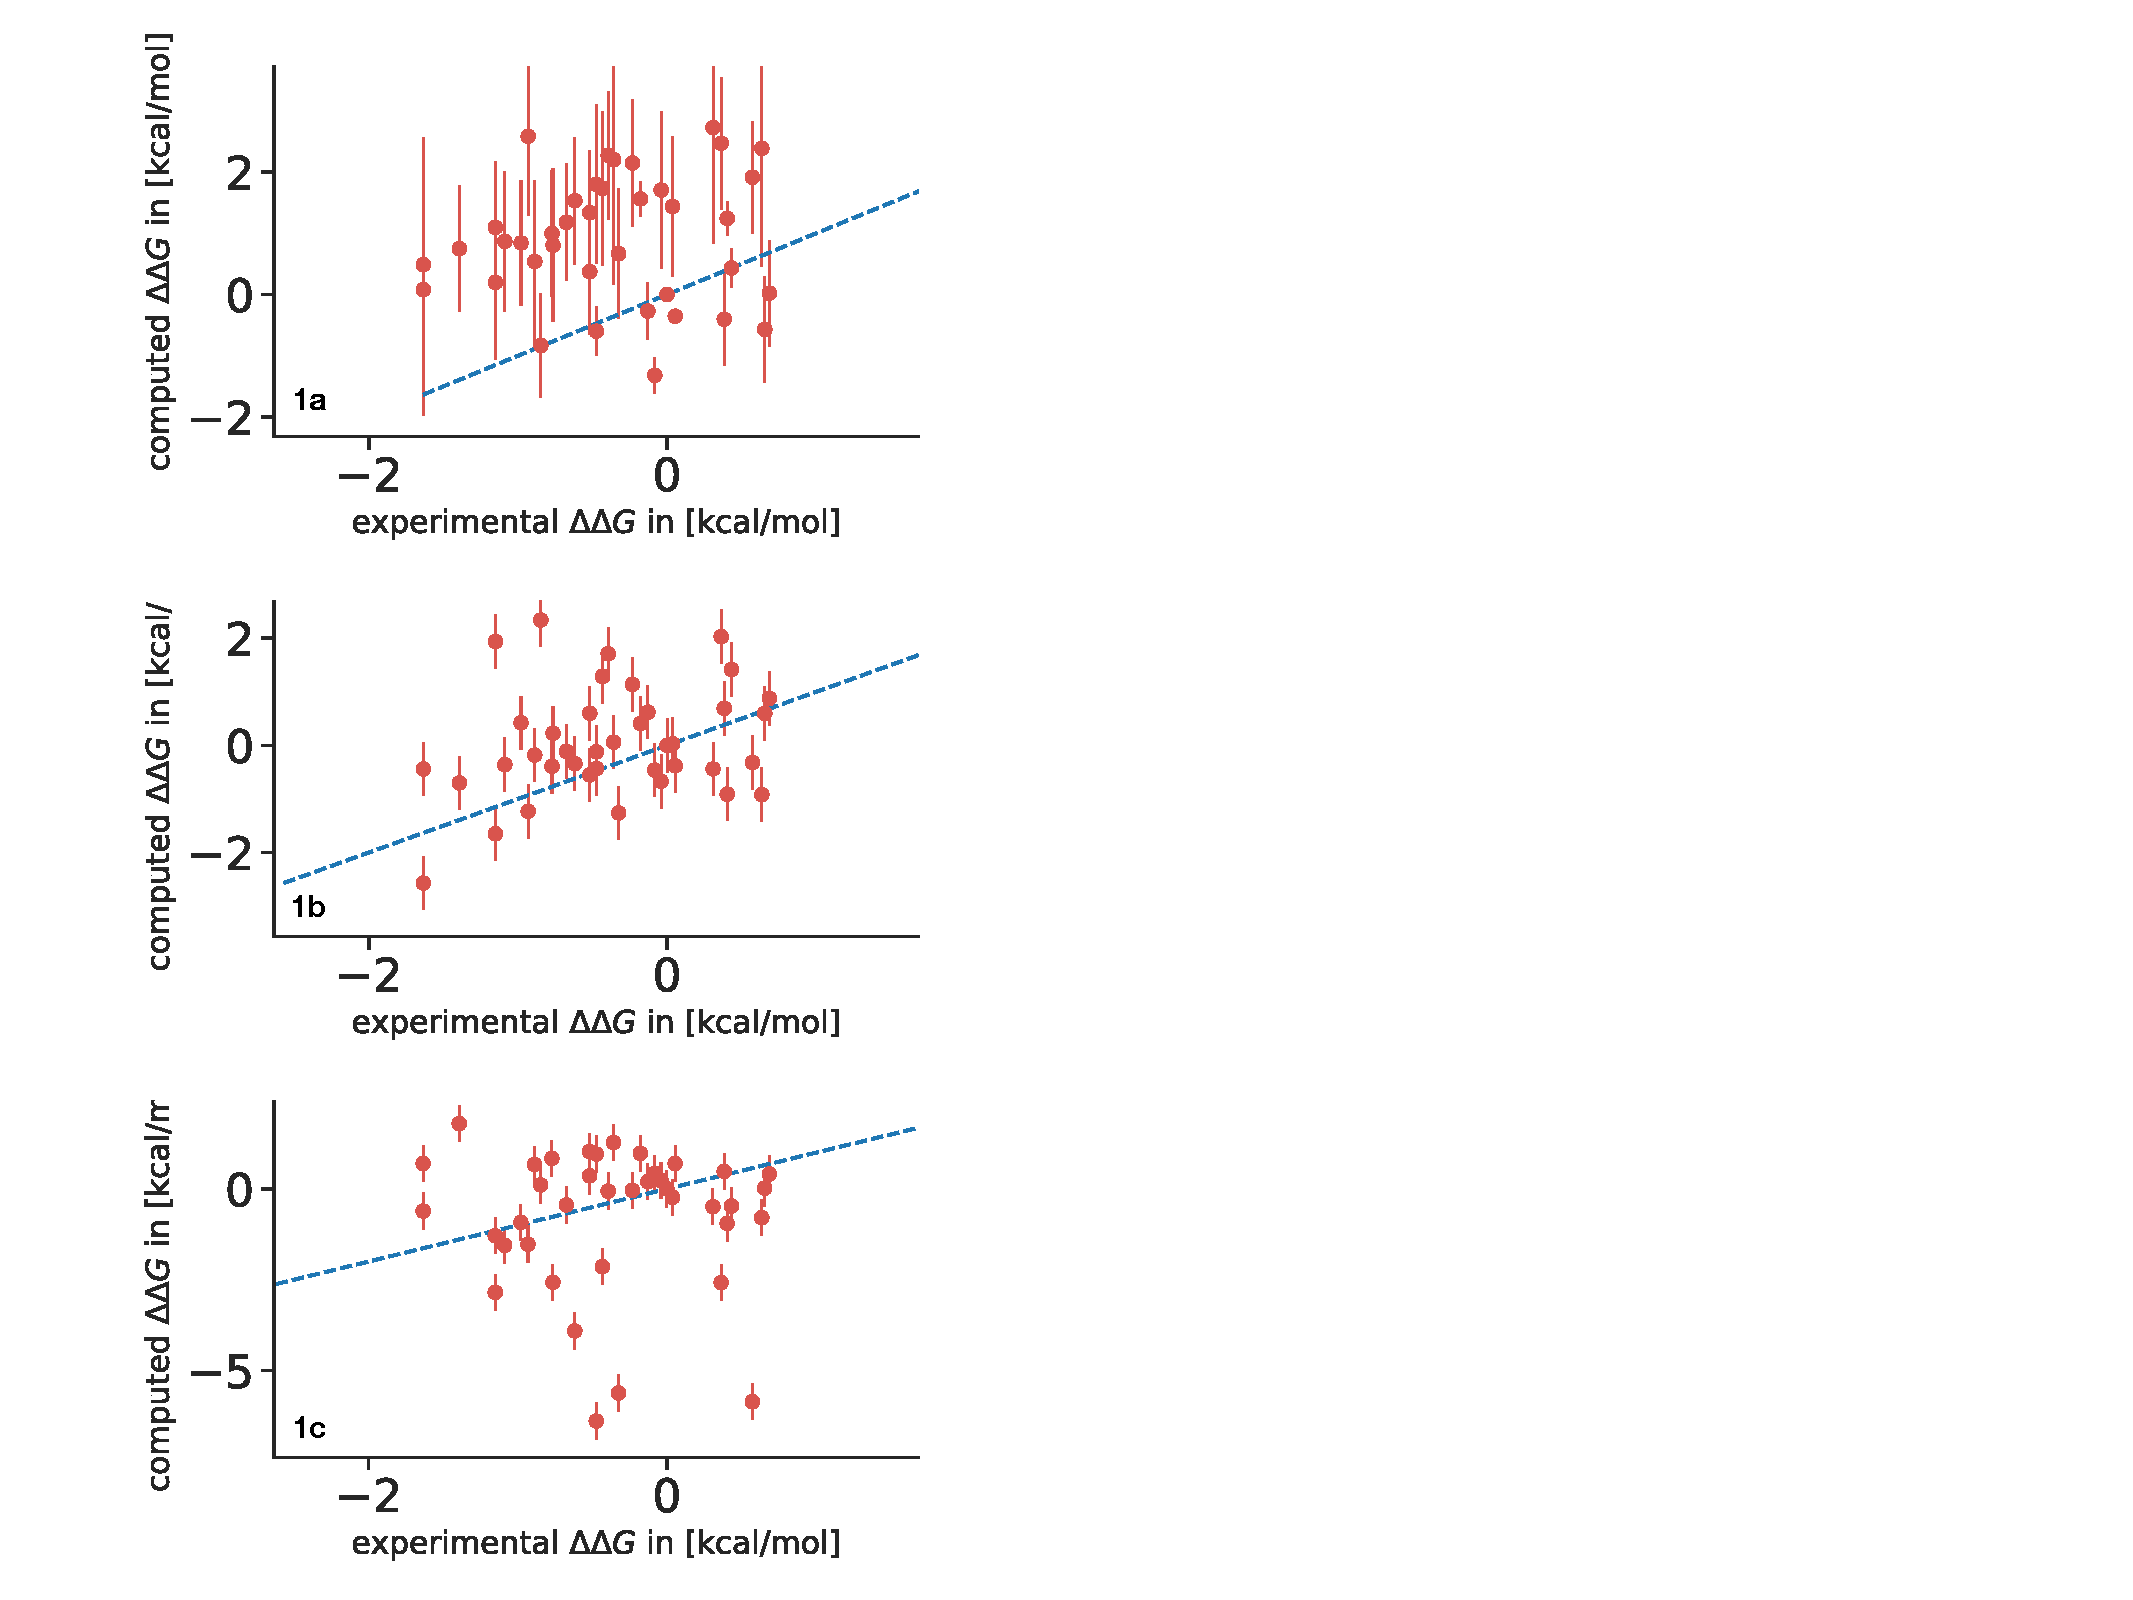
\includegraphics[width=\columnwidth]{figures/Fig1/Fig1.pdf}
\caption{\label{fig:fig1} (a) Binding free energy prediction from SOMD free energy estimate with respect to experimental data computed from IC 50s (b) Binding free energy prediction from Docked compounds with Flare compared to experiments (c) Binding free energy predictions from structures aligned to crystal pose using Flare for scoring }
\end{figure}
\begin{table}[]
\begin{tabular}{|l|lll}
\hline
              & \multicolumn{1}{l|}{R} & \multicolumn{1}{l|}{$\tau$} & \multicolumn{1}{l|}{MUE in kcal/mol} \\ \hline
SOMD          & 0.05 $\pm$0.14         & 0.003 $\pm$0.16             & 1.6 $\pm$ 0.2                        \\ \cline{1-1}
Flare Docking & 0.2 $\pm$ 0.1          & 0.1 $\pm$0.1                & 1.0 $\pm$ 0.1                        \\ \cline{1-1}
Flare Crystal & -0.05 $\pm$0.04        & -0.003 $\pm$0.070           & 1.5 $\pm$0.1                         \\ \hline
\end{tabular}
\caption{\label{tab:tab1}}
\end{table}
\section{Discussion and conclusions}

All the discussions. 



\section{Author Contributions}
%%%%%%%%%%%%%%%%
% This section mustt describe the actual contributions of
% author. Since this is an electronic-only journal, there is
% no length limit when you describe the authors' contributions,
% so we recommend describing what they actually did rather than
% simply categorizing them in a small number of
% predefined roles as might be done in other journals.
%
% See the policies ``Policies on Authorship'' section of https://livecoms.github.io
% for more information on deciding on authorship and author order.
%%%%%%%%%%%%%%%%

(Explain the contributions of the different authors here)

% We suggest you preserve this comment:
For a more detailed description of author contributions,
see the GitHub issue tracking and changelog at \githubrepository.

\section{Other Contributions}
%%%%%%%%%%%%%%%
% You should include all people who have filed issues that were
% accepted into the paper, or that upon discussion altered what was in the paper.
% Multiple significant contributions might mean that the contributor
% should be moved to authorship at the discretion of the a
%
% See the policies ``Policies on Authorship'' section of https://livecoms.github.io for
% more information on deciding on authorship and author order.
%%%%%%%%%%%%%%%

(Explain the contributions of any non-author contributors here)
% We suggest you preserve this comment:
For a more detailed description of contributions from the community and others, see the GitHub issue tracking and changelog at \githubrepository.

\section{Potentially Conflicting Interests}
%%%%%%%
%Declare any potentially competing interests, financial or otherwise
%%%%%%%

Declare any potentially conflicting interests here, whether or not they pose an actual conflict in your view.

\section{Funding Information}
%%%%%%%
% Authors should acknowledge funding sources here. Reference specific grants.
%%%%%%%
FMS acknowledges the support of NSF grant CHE-1111111.

\bibliography{livecoms-sample}

%%%%%%%%%%%%%%%%%%%%%%%%%%%%%%%%%%%%%%%%%%%%%%%%%%%%%%%%%%%%
%%% APPENDICES
%%%%%%%%%%%%%%%%%%%%%%%%%%%%%%%%%%%%%%%%%%%%%%%%%%%%%%%%%%%%

%\appendix


\end{document}
